\documentclass[a4paper,12pt]{article} 

%%% Работа с русским языком
\usepackage{cmap}                           % поиск в PDF
\usepackage{mathtext} 			 	       % русские буквы в формулах
\usepackage[T2A]{fontenc}               % кодировка
\usepackage[utf8]{inputenc}              % кодировка исходного текста
\usepackage[english,russian]{babel}  % локализация и переносы

%Матеша
\usepackage{amsmath,amsfonts,amssymb,amsthm,mathtools} % AMS
\usepackage{icomma} % "Умная" запятая

%\mathtoolsset{showonlyrefs=true} % Показывать номера только у тех формул, на которые есть \eqref{} в тексте.

%% Шрифты
\usepackage{euscript}	 % Шрифт Евклид
\usepackage{mathrsfs} % Красивый матшрифт

%% Свои команды
\DeclareMathOperator{\sgn}{\mathop{sgn}}

%% Перенос знаков в формулах (по Львовскому)
\newcommand*{\hm}[1]{#1\nobreak\discretionary{}
{\hbox{$\mathsurround=0pt #1$}}{}}

\usepackage{geometry}
 \geometry{
 a4paper,
 top=25mm,
 }





\usepackage{graphicx}
\usepackage{amsmath,amsfonts,amssymb,amsthm,mathtools} % AMS
\usepackage{icomma} % "Умная" запятая

%\mathtoolsset{showonlyrefs=true} % Показывать номера только у тех формул, на которые есть \eqref{} в тексте.

%% Шрифты
\usepackage{euscript}	 % Шрифт Евклид
\usepackage{mathrsfs} % Красивый матшрифт




\begin{document}
    \begin{titlepage}
    \begin{center}
        \vspace{4cm}
        \huge {\textbf{Отчет о выполнении лабораторной работы 1.2.2}}
        {} \\
        \vspace{1cm}
        \Large {\textbf{Экпериментальная проверка закона}} \\
        \Large {\textbf{вращательного движения}} \\
        \Large {\textbf{на крестообразном маятнике}} \\

        \vspace{10cm}
        \begin{flushright}
        \begin{minipage}{.45\textwidth}
        \normalsize{\textbf{Студент:} Копытова Виктория Сергеевна}\\
        \textbf{Группа:} Б03-304\\
        \end{minipage}
        \end{flushright}

        
    \end{center}
    \end{titlepage}
	\newpage






\section {Аннотация}
\textbf{Цель работы:} Экпериментально получить зависимость углового ускорения от момента прикладываемых к маятнику сил, убедиться, что угловое ускорение зависит линейно от момента сил, определить момент инерции маятника; проанализировать влияние сил трения, дейтвующих на ось вращения\\
\\
\textbf{В работе используются:} крестообразный маятник, набор перегрузков, секундомер, линейка, штангенциркуль.
\\


\section{Теоретические сведения}
Основное уравнение вращательного движения тела вокруг закреплённой оси:
\begin{equation}\label{1}
I \ddot{\varphi} = M, 
\end{equation}
где $\ddot{\varphi} \equiv \dot{\omega} \equiv \beta$ -- угловое ускорение ($\omega$  -- угловая скорость), $I$ -- полный момент инерции тела относительно оси вращения, $M$ -- суммарный момент внешних сил относительно этой оси.

\subparagraph*{Цель работы:} экспериментально проверить уравнение \eqref{1}, получив зависимость углового ускорения от момента инерции и момента прикладываемых к системе сил, а также проанализировать влияние сил трения, действующих в оси вращения.
\subparagraph*{Экспериментальная установка:} для экспериментального исследования закона вращательного движения \eqref{1} в работе используется крестообразный «маятник» ,  устройство которого изображено на рис. \ref{fig:image}. Маятник состоит из четырёх тонких стержней радиуса $a$, укреплённых на втулке под прямым углом друг к другу. Втулка и два шкива различных радуисов  ($r_1$ и $r_2$) насажены на общую ось. Ось закреплена в подшипниках, так что вся система может свободно вращаться вокруг горизонтальной оси. Момент инерции  {$I$} маятника можно изменять, передвигая грузы $m_i (i = 1, \dots, 4)$ вдоль стержней и меняя $R_i$. На один из шкивов маятника навита тонкая нить. Привязанная к ней лёгкая платформа известной массы $m_п$ служит для размещения перегрузков $m_г$. 

Установка оснащена датчиком, позволяющим фиксировать моменты времени прохождения концов стержней через него. Данные с датчика передаются на компьютер для последующей обработки и получения зависимостей угла поворота $\varphi(t)$, угловой скорости $\omega \equiv \dot{\varphi}$ и углового ускорения маятника $\beta \equiv \ddot{\varphi}$ от времени, а также углового ускорения от угловой скорости $\beta(\omega)$.

\begin{figure}[h]
	\center{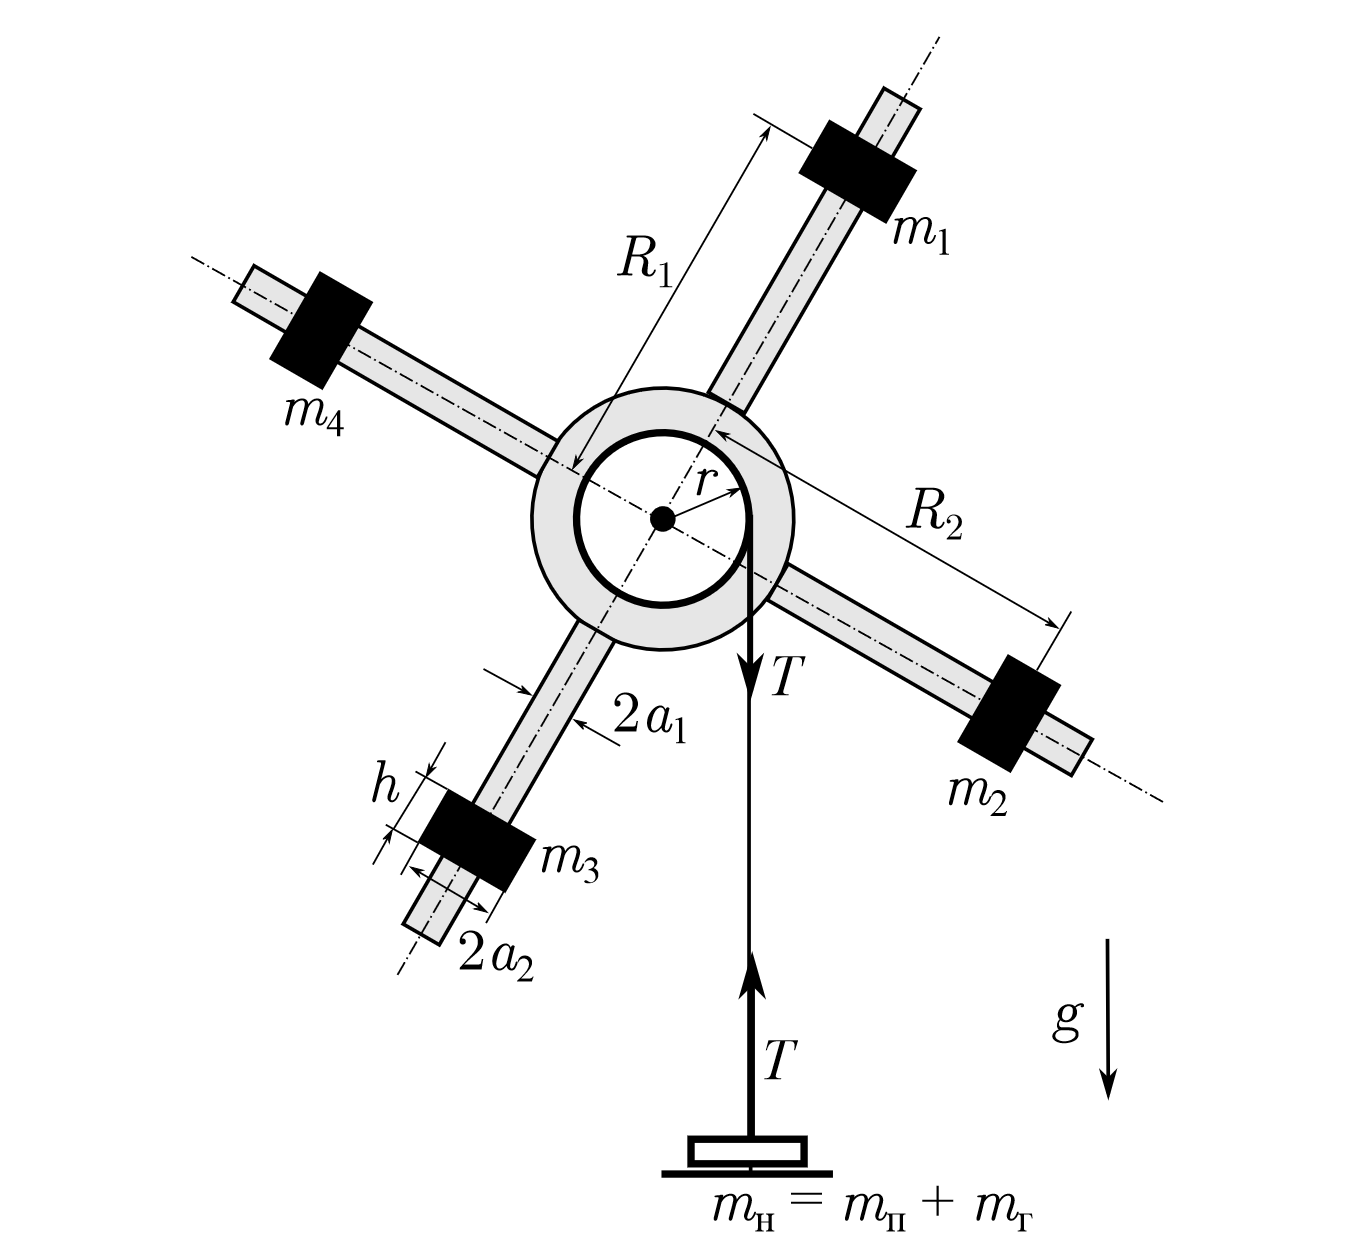
\includegraphics[scale=0.35]{обербек.png}}
	\caption{Схема установки}
	\label{fig:image}
\end{figure}



\subparagraph*{Вывод уравнения движения маятника: } рассмотрим силы, действующие на маятник. Основной вращающий момент поздаётся подвешенным на нити перегрузком. Непосредственно на маятник действует момент силы натяжения нити: $M_н = rT$, где $r$ -- радиус шкива ($r_1$ или $r_2$). Силу $T$ выразим из уравнения движения платформы $m_н\ddot{y}= m_нg - T$, где $m_н = m_п + m_г$ -- масса платформы с перегрузком. Ускорение платформы связано с угловым ускорением маятника условием нерастяжимости нити $\ddot{y}=\beta r$. Отсюда момент силы натяжения нити 
\begin{equation}\label{2}
M_н = m_нr(g - \beta r).
\end{equation}
Вращению маятника препятствует момент силы трения в оси  $M_{тр}$. Таким образом, с учётом \eqref{2} уравнение  \eqref{1} может быть записано как
\begin{equation}\label{3}
(I + m_нr^2)\beta = m_нgr - {M_{тр}}.
\end{equation}
Заметим, что в наших опытах, как правило, $m_нr^2 \ll I$, и соответственно $M_н \approx m_нgr$, то маятник будет раскручиваться с постоянным угловым ускорением $\beta _0 \approx m_нgr / I$.

Поскольку зависимость момента силы трения от нагрузки на маятник и скорости его вращения не известна (её исследование -- отдельная экспериментальная задача), методика измерения должна быть построена так, чтобы минимизировать или вовсе исключить влияние $M_{тр}$. Можно высказать следующие качественные соображения о природе и величине $M_{тр}$. Она может иметь как составляющую, пропорциональную силе реакции в оси $N$ (сухое трение в подшипниках),  так и составляющую, пропорциональную угловой скорости $\omega$ вращения маятника (вязкое трение в подшипниках и сопротивления воздуха). Учитывая, что сила реакции уравновешенного маятника равна $N = m_мg + T \approx (m_м + m_н)g \approx m_мg $, где $m_м$ -- масса маятника (как правило, $m_м \gg m_н$), можно записать
\begin{equation}\label{4}
M_{тр} \simeq \left(1 + \frac{m_н}{m_м}\right)M_0 + \eta\omega \approx M_0 + \eta\omega,
\end{equation}
где $M_0$ -- момент сил трения для покоящегося маятника при нулевой массе подвеса (минимальное значение силы трения), $\eta$ -- некоторый коэффициент, отвечающий за вязкое трение.
\subparagraph*{Методика эксперимента:}малость величины трения $M_{\text{тр}}$ в работе обеспечивается за счёт использования в креплении подшипников качения. Однако учёт трения всё же оказывается необходим, поскольку оно существенно влияет на результаты опыта как при малых массах перегрузков (когда $m_{г} \sim M_0 / gr$), так и при больших, поскольку при увеличении $m_{н}$ возрастает сила реакции в оси и угловая скорость вращения маятника, а с ней и вязкое трение.

Влияние вязкой составляющей трения можно исключить следующим образом. Экспериментальная установка позволяет измерять зависимость углового ускорения от угловой скорости $\beta (\omega)$. Если верны предположения о малости величины силы трения,то угловое ускорение должно быть линейной функцией угловой скорости:
\begin{equation}
    \beta (\omega) = \beta_0 + k\omega
\end{equation}

\section{Ход работы} 
Величины, характерные для используемого маятника:
\begin{table}[h]
    \centering
    \begin{tabular}{|c|c|}
        \hline
        Радиус малого шкива $r_{\text{м}}$, см & 0.9 \\
        \hline
        Радиуc большого шкива $r_{\text{б}}$, см & 1.5 \\
        \hline
        Масса платформы $m_{\text{п}}$, г & 6.17 \\
        \hline
    \end{tabular}
    \caption{Характеристики маятника}
\end{table}
\begin{enumerate}
    \item Расположим грузы на расстоянии $R=3.1$ см и проведём балансировку маятника.
    \item Оценим момент силы трения в подшипниках.
    Маятник начинает двигаться, когда на плотформе находится груз массой $m_{\text{гр}}=6.45$ граммов. Измерение проводится на малом шкиве.
    Тогда момент силы трения:
    \begin{displaymath}
        M_{\text{тр}} = (m_{\text{гр}}+m_{\text{п}})g \cdot r_{\text{м}} \approx 1.11 \cdot 10^{-3} (Н \cdot м) 
    \end{displaymath}
    \item При фиксированной массе перегрузка и моменте инерции маятника проведём измерения для вычисления случайной погрешности измерения $\beta_0$. Данные представлены в таблице 2.
    \begin{table}[h]
        \centering
        \begin{tabular}{|c|c|c|}
            \hline
            $k$, 1/c & $\beta_0$, рад/$c^2$ & ($\beta_{0сред}$ -$ \beta_{0i})^2, рад^2 / c^4 $ \\ \hline
	        $ -0.0078\pm 0.0058$ & $ 0.5126\pm 0,0012 $ & 0.0015 \\
        	$ -0.0079\pm 0.0045$ & $ 0.4388\pm 0.0018$ & 0.0012 \\
        	$ -0.0085\pm 0.0070$ & $ 0.4737\pm 0.0016 $ & 0.0001\\
        	$ -0.0084\pm 0.0015$ & $ 0.4999\pm  0.0014$  & 0.0007\\
        	$ -0,0088\pm 0.0049$ & $ 0.4749\pm 0.0039$ & 0.0001\\ 
            \hline
        \end{tabular}
        \caption{Оценка случайной погрешности $\beta_0$}
    \end{table}
    \begin{displaymath}
        \beta_{0сред} \approx 0.4800 (рад/с^2)
    \end{displaymath}
    \begin{displaymath}
        \sigma_{случ}= \sqrt{ \frac{\sum\limits_{i=1}^n (\beta_{0сред} - \beta_{0n})^2}{n(n-1)}} \approx 0.01 \quad рад / c^2
    \end{displaymath}
    \item Проведём опыт для разных масс грузов. Вычислим моменты силы натяжения нити $M_Т = (m_г+m_п)gr_{б,м}$. Полученные данные занесём в таблицу 3.
    \begin{table}[h]
        \centering
        \begin{tabular}{|c|c|c|c|c|}
            \hline
            $m_г, г$ & $k, 1/c$& $\beta_0, рад/c^2$ & Радиус шкива $r_{б, м}, см$ & $ M_T, мН \cdot м $ \\ 
            \hline
            62.9 & $-0.0113 \pm 0.0021 $ & $ 0.669  \pm 0.002  $ & 1.78 & 12.0 \\
        	100  & $ -0.0123\pm 0.0022 $ & $ 1.067  \pm 0.007  $ & 1.78 & 18.5 \\
        	200  & $ -0.0253\pm 0.0041 $ & $ 2.300  \pm 0.008  $ & 1.78 & 36.0 \\
        	100  & $ -0.0200\pm 0.0076 $ & $ 0.6034 \pm 0.0048 $ & 0.90 & 9.4  \\
        	62.9 & $ -0.0161\pm 0.0053 $ & $ 0.3482 \pm 0.0019 $ & 0.90 & 6.1 \\ 
            \hline
        \end{tabular}
        \caption{Измерения $k$ и $\beta_0$ для разных масс грузов}

    \end{table}
    Построим график зависимости $\beta_0(M_T)$:
    \begin{figure}[h]
        \centering
        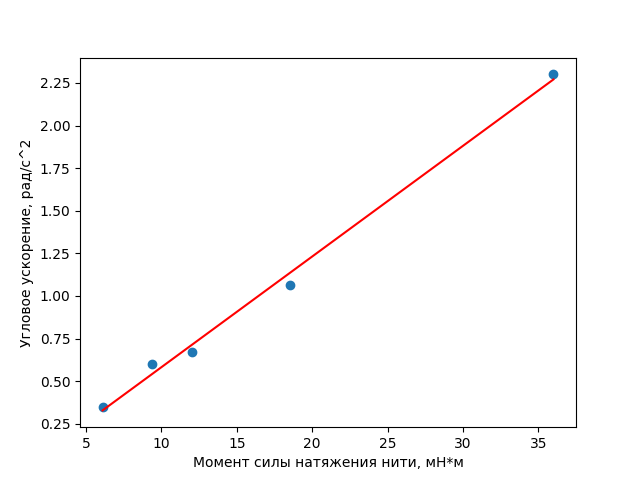
\includegraphics[scale = 0.8]{1.png}
        \caption{Линейная зависимость $\beta_0(M_T)$}
        \label{fig:enter-label}
    \end{figure}
        
        Мы видим, что зависимость линейная, значит:
        \begin{displaymath}
            \beta_0 = a + b \cdot M_T
        \end{displaymath}
    Вычислим коэффициенты a и b по методу наименьших квадратов:
    \begin{displaymath}
        a = -0.068 \quad рад/c^2
    \end{displaymath}
    \begin{displaymath}
        b = 64.95 \quad 1/кг \cdot м^2
    \end{displaymath}

    При пересечении с осью абсцисс:
    \begin{displaymath}
        M_T = -\frac{a}{b} \approx 1.05 \cdot 10^{-3} \quad Н \cdot м
    \end{displaymath}
    Момент инерции:
    \begin{displaymath}
        I = \frac{1}{b} \approx 15.0 \cdot 10^{-3} \quad кг \cdot м^2
    \end{displaymath}
    Погрешность вычисления момента инерции:
    \begin{displaymath}
        \varepsilon_b = \varepsilon_I
    \end{displaymath}
    \begin{displaymath}
        \sigma_b = \dfrac{1}{\sqrt{n}}\sqrt{\dfrac{\left\langle \beta_0^2\right\rangle - \left\langle \beta_0\right\rangle^2}{\left\langle \
		M_Т^2\right\rangle - \left\langle М_Т\right\rangle^2} - b^2} \approx 1.98 \quad (1/кг\cdot м^2)
    \end{displaymath}
    \begin{displaymath}
        \varepsilon_b = \frac{\sigma_b}{b} \approx 0.03
    \end{displaymath}
    \begin{displaymath}
        \sigma_I = \varepsilon_I I = \varepsilon_b I \approx 0.46 \cdot 10^{-3}
    \end{displaymath}
    Окончательно:
    \begin{displaymath}
        I = (15.0 \pm 0.46) \cdot 10^{-3} \quad кг \cdot м^2
    \end{displaymath}
    \item Определим зависимость углового ускорения от момента инерции системы, данные занесём в таблицу. Из формулы (5) вычислим
    \begin{displaymath}
        I  = \dfrac{m_нgr - M_{тр}}{\beta}  - m_н r^2 \approx \dfrac{m_нgr - M_{тр}}{\beta}, \quad I \gg m_н r^2
    \end{displaymath}
    \begin{table}[h]
        \centering
        \begin{tabular}{|c|c|c|c|}
            \hline
            $R, см$ & $k, 1/c$ & $\beta, рад/с^2$ & $I, кг\cdot м^2 \cdot 10^{-3}$ \\ 
            \hline
            3 & -0.379 & 1.192 & 7.00\\
            5 & -0.307 & 0.987 & 8.51\\
            8 & -0.319 & 0.715 & 11.64\\
            \hline
        \end{tabular}
        \caption{Зависимость углового ускорения от момента инерции системы}
    \end{table}
    
    Построим график зависимости $I(R^2)$:
    \begin{figure}[h]
        \centering
        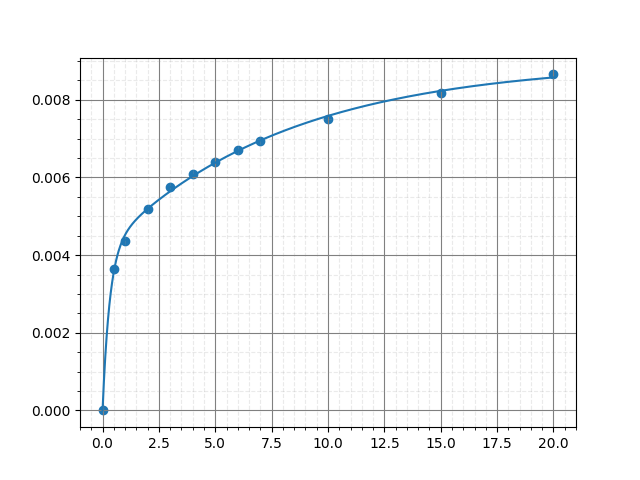
\includegraphics[scale = 0.8]{2.png}
        \caption{Линейная зависимость $I(R^2)$}
    \end{figure}

    Зависимость линейная, значит
    \begin{displaymath}
        I = a + b R^2
    \end{displaymath}
    Методом наименьших квадратов вычислим коэффициенты a и b:
    \begin{displaymath}
        a = 0.0063 \quad кг \cdot м^2
    \end{displaymath}
    \begin{displaymath}
        b = 0.8360 \quad кг
    \end{displaymath}
    \begin{displaymath}
        \sigma_b = \dfrac{1}{\sqrt{n}}\sqrt{\dfrac{\left\langle I^2 \right\rangle - \left\langle I \right\rangle^2}{\left\langle \
		R^4\right\rangle - \left\langle R^2\right\rangle^2} - b^2} \approx 0.018 \quad кг
    \end{displaymath}
    \begin{displaymath}
        \sigma_a = \sigma_b \sqrt{\left\langle R^4 \right\rangle - \left\langle R^2 \right\rangle ^2 } \approx 3.2 \cdot 10^{-5} \quad кг \cdot м^2
    \end{displaymath}
    Момент инерции можно вычислить по формуле 
    \begin{displaymath}
        I = I_0 + \sum\limits_{i = 1}^4{(I_i + m_iR_i^2)},
    \end{displaymath}
    где $I_0$ -- момент инерции маятника без дополнительных грузов, $m_i$ -- масса этого дополнительного груза, $I_i$ -- его момент инерции относительно центра масс системы.

    Тогда
    \begin{displaymath}
        I_0 = a = (6.3 \pm 0.03) \cdot 10^{-3} \quad кг \cdot м^2
    \end{displaymath}
    \item Найдём $I_0$, измеряя коэффициент $\beta_0$ для маятника без дополнительных грузов на маленьком шкиве. Занесём данные в таблицу.
    \begin{table}[h]
        \centering
        \begin{tabular}{|c|c|c|c|}
            \hline
            $m_г$, г & $k, 1/c$ & $\beta_0$, $рад/c^2$ & $I_0 кг\cdot м^2 \cdot 10^{-3}$  \\
            \hline
            100 & $-0.0 452 \pm 0.0031$ & $ 1.328 \pm 0.006 $ & 6.27 \\
            100 & $-0.0407  \pm 0.0056$ & $ 1.389 \pm 0.009 $ & 5.99 \\
            100 & $-0.0839  \pm 0.001 $ & $ 1.331 \pm 0.008 $ & 6.25 \\ 
            \hline
        \end{tabular}
        \caption{Измерение $I_0$}
    \end{table}
    \begin{displaymath}
        I_0 = \frac{(m_п+m_г)gr_м - M_0}{\beta_0}
    \end{displaymath}
    \begin{displaymath}
        \left\langle I_0 \right\rangle = 6.17 \cdot 10^{-3} \quad кг\cdot м^2 
    \end{displaymath}
\end{enumerate}



\section{Вывод}

\subparagraph*{}В ходе работы была получена зависимость углового ускорения маятника от его момента инерции и момента прикладываемых сил. Угловое ускорение прямо пропорционально моменту сил и обратно пропорционально моменту инерции. Был оценён вклад силы трения в оси вращения в общий момент прикладываемых сил, а также погрешности вычислений. Двумя разными способами был вычислен момент инерции маятника без грузов и оба метода дали приблизительно одинаковый результат, что доказывает справедливость использованных в работе теоретически полученных зависимостей.




\end{document}